%---A LaTeX template for Mechatronics ME 495 Capstone report.
\documentclass[twocolumn]{article}
\oddsidemargin=-0.35in
\topmargin=-0.75in
\headsep=0.1667in
\columnsep=0.25in
\textwidth=7.25in
\textheight=9.125in
\headheight=12pt

\usepackage{myfontstyle}			% Palatino & Euler fonts
\usepackage{graphicx}               % begin standard LaTeX macros
\usepackage{fancyhdr}               % fancy headers, see fancyhdr.pdf
\usepackage{fancyvrb}               % fancy verbatim environment, see fancyvrb.pdf
\usepackage{lastpage}               % used in the footer to specify the last page
\usepackage{amsmath}                % for log-like symbols
\usepackage{color}
\usepackage{dtklogos}
\usepackage{listings}
\newcommand{\bra}[1]{\langle #1|}
\newcommand{\ket}[1]{|#1\rangle}
\newcommand{\braket}[2]{\langle #1|#2\rangle} 

\begin{document}	%  <--- Here is where the document starts

\title{
	\vspace{-0.5in}\rule{\textwidth}{1pt}
	\begin{tabular}{ll}\begin{minipage}{4.75in}\vspace{6px}
			\noindent\Large Department of Mechanical Engineering\\
			\vspace{-12px}\\
			\noindent\large University of Washington\qquad 
		\end{minipage}&\begin{minipage}{2in}\vspace{6px}\small
		Stevens Way, Box 352600\\
		Seattle, WA 98195 USA\\
		206-543-5090
	\end{minipage}\end{tabular}
	\rule{\textwidth}{1pt}\vspace{0.25in}
	\Large
	Mechanical Impedance Control
}

\date{Mechatronics Capstone Design Report --- June 10, 2016}

\author{
	{Richard S Chen}\\
	rchen3@uw.edu
	\and 
	{Nathan Robert Dabling}\\
	ndabling@uw.edu
	\and
	{Fangzhong Guo}\\
	fzguo@uw.edu
	\and
	{James Kurniawan}\\
	kurnij@uw.edu
	\and
	{Kyle R Spangenberg}\\
	spangkyl@uw.edu
	\and
	{Advising Professor}\\
	Prof. Joseph L. Garbini
}

\maketitle


%---Executive Summary
\subsection*{Executive Summary{{\color{red}\ *}}}

Here is a suggested outline for Mechatronics ME 495 reports. Since the projects of all groups are different, feel free to modify the organization of this format to meet your project requirements. However, note that some sections ({\color{red}\bf{*}}) are required. 

%---Introduction
\subsection*{Introduction}

\subsubsection*{---Problem Definition} \par
The main goal of this project is to demonstrate the viability of a variable impedance controller with the use of a one-dimensional prototype. Variable impedance control utilizes user input in order to achieve a desired state of mobility. The system senses a force and responds by changing its impedance to match the desired input parameters of the user. The user will be able to control the virtual weight, damping, and spring force. These virtual parameters will dictate how the system performs while being used. \par
There are many applications for this research and while only a simple prototype, the implications are far-reaching. With variable impedance control, a heavy object can feel lighter and be easier to maneuver. Lighter objects that don't provide enough feedback for a human can have their apparent weight increased. When human control and reasoning is desired over robot logic, variable impedance control can make a difference. This report details the design and construction of a one-dimensional cart prototype that successfully demonstrates the capability of a variable impedance controller.\par

\subsubsection*{---Functional Requirements} \par
At the beginning of the design phase, target values for the settling time and percent overshoot were set, found in \ref{specs}.
\begin{table}[H]
	\centering
	\caption{Functional Specifications}
	\label{specs}
	\begin{tabular}{|l|l|}
		\hline
		Target Requirement &          \\ \hline
		\%OS               & 5\%      \\ \hline
		Settling Time      & 0.15 sec \\ \hline
	\end{tabular}
\end{table}
Using the targets, an appropriate motor and amplifier were attained. In selecting a motor, a reference had to be used to run simulations, so a motor with a torque constant of .11 N/m was used in tandem with an amplifier with a gain of .79 A/V. Using these sample motor and amplifier constants in the model, simulations were run through Simulink to verify that such a motor and amplifier combination would suffice by checking the maximum current, voltage, torque and rpm required against what the motor and amp could supply. Cases with low mass and damping proved to have the highest torque and current requirements because the velocity profile of such a system would involve very high accelerations. From the results we decided that damping must always be included in the reference system to limit the necessary torque. \par
After the design was finalized a functional specification map was created to guide the user's inputs. The motivation for this was observing that the low mass, low damping case performed reasonably well as long as the force input was small. In addition, a greater force could be applied if either the damping or mass was increased. This led to the conclusion that the limitations on the reference system parameters were actually coupled. Considering the restrictions that either increasing the mass or the damping would put on the acceleration of the reference system for a given force input, this conclusion seemed logical. To create the mapping, the transfer function relating the force input to the required motor current was calculated.
\begin{figure*}
	\includegraphics[width=1\linewidth]{Images/Functional_Specifications_Mapping}
	\caption{3D mapping of the maximum human input force for varying virtual mass and damping. Virtual stiffness is set to 5 N/m}
	\label{fig:Functional_Specifications_Mapping}
\end{figure*}
\begin{equation}
I = \frac{[K_{P}s+K_{I}][(\epsilon-M)s^{2}-Bs-K]}{[\frac{\epsilon}{K_{A}}s^{2}+\frac{K_{P}K_{M}}{r}s+\frac{K_{I}K_{M}N}{r}][Ms^{2}+Bs+K]}F
\end{equation}
Where 
\begin{equation}
\epsilon = M+\frac{JN^{2}}{r^{2}}
\end{equation}
\newline \indent The transfer function depends on the parameters of both the reference and actual systems, as predicted, but not in any clearly identifiable way. The mapping was generated numerically using successive approximation to determine what applied force would result in the current requirement exceeding the limitations of the amplifier, about 4.8 A. The parameters varied were the mass and damping, as the relationship between the spring and acceleration was less complex and more intuitive and the input force was a critical component of any mapping.
\newline \indent The mapping shown in Figure 1 is just a small portion of the effective range. This portion was selected because it demonstrates the very small force that can be applied when the reference system has very low mass. The maximum value of force shown is near 111 N which is approximately the limit of the load cell range. Theoretically, the force possible to apply would continue to increase beyond this point but the load cell would not read it as a greater force, so the system cannot handle greater forces regardless. If the load cell range was not the limiting factor, it is presumed that the force would increase with the damping and mass until the torque required to prevent the acceleration of the real system going beyond the reference system's response for the input force. In this way, the lower range of the the functional specification mapping can be seen as dependent on the ability of the motor to increase the acceleration of the real system and the higher range of the functional specification mapping can be seen as dependent on the ability of the motor to decrease the acceleration of the real system.


%---The Design
\subsection*{The Design}

\subsubsection*{ ---Description}
The goal of the impedance controller was to force the response of a relatively simple reference system onto a very different, more complex real system. The real system was a linear actuator connected to a motor through a belt drive and powered by the myRIO microcomputer's control signal amplified through a current amplifier. 

The reference system simulated by the impedance controller was an ideal mass, spring, damper system all in parallel with a force input. The continuous time transfer function was found using normal tree state equation formulation. The continuous time transfer function was discretized into a single biquad using Tustin's approximation. This approximation was calculated by hand in order to find the symbolic relationships between the coefficients of the transfer function and the parameters set by the user. This was crucial to enable the user to adjust the mass, stiffness and damping of the system while the program ran instead of closing out and rerunning a MATLAB script to recalculate the biquad structure. The results of the hand calculation were verified using MATLAB before testing began. 
%At the beginning of the design phase, target values for the settling time and percent overshoot were set, found in \ref{specs}.
\begin{table}[H]
	\centering
	\caption{Functional Specifications}
	\label{specs}
	\begin{tabular}{|l|l|}
		\hline
		Target Requirement &          \\ \hline
		\%OS               & 5\%      \\ \hline
		Settling Time      & 0.15 sec \\ \hline
	\end{tabular}
\end{table}
Using the targets, an appropriate motor and amplifier were attained. In selecting a motor, a reference had to be used to run simulations, so a motor with a torque constant of .11 N/m was used in tandem with an amplifier with a gain of .79 A/V. Using these sample motor and amplifier constants in the model, simulations were run through Simulink to verify that such a motor and amplifier combination would suffice by checking the maximum current, voltage, torque and rpm required against what the motor and amp could supply. Cases with low mass and damping proved to have the highest torque and current requirements because the velocity profile of such a system would involve very high accelerations. From the results we decided that damping must always be included in the reference system to limit the necessary torque. \par
After the design was finalized a functional specification map was created to guide the user's inputs. The motivation for this was observing that the low mass, low damping case performed reasonably well as long as the force input was small. In addition, a greater force could be applied if either the damping or mass was increased. This led to the conclusion that the limitations on the reference system parameters were actually coupled. Considering the restrictions that either increasing the mass or the damping would put on the acceleration of the reference system for a given force input, this conclusion seemed logical. To create the mapping, the transfer function relating the force input to the required motor current was calculated.
\begin{figure*}
	\includegraphics[width=1\linewidth]{Images/Functional_Specifications_Mapping}
	\caption{3D mapping of the maximum human input force for varying virtual mass and damping. Virtual stiffness is set to 5 N/m}
	\label{fig:Functional_Specifications_Mapping}
\end{figure*}
\begin{equation}
I = \frac{[K_{P}s+K_{I}][(\epsilon-M)s^{2}-Bs-K]}{[\frac{\epsilon}{K_{A}}s^{2}+\frac{K_{P}K_{M}}{r}s+\frac{K_{I}K_{M}N}{r}][Ms^{2}+Bs+K]}F
\end{equation}
Where 
\begin{equation}
\epsilon = M+\frac{JN^{2}}{r^{2}}
\end{equation}
\newline \indent The transfer function depends on the parameters of both the reference and actual systems, as predicted, but not in any clearly identifiable way. The mapping was generated numerically using successive approximation to determine what applied force would result in the current requirement exceeding the limitations of the amplifier, about 4.8 A. The parameters varied were the mass and damping, as the relationship between the spring and acceleration was less complex and more intuitive and the input force was a critical component of any mapping.
\newline \indent The mapping shown in Figure 1 is just a small portion of the effective range. This portion was selected because it demonstrates the very small force that can be applied when the reference system has very low mass. The maximum value of force shown is near 111 N which is approximately the limit of the load cell range. Theoretically, the force possible to apply would continue to increase beyond this point but the load cell would not read it as a greater force, so the system cannot handle greater forces regardless. If the load cell range was not the limiting factor, it is presumed that the force would increase with the damping and mass until the torque required to prevent the acceleration of the real system going beyond the reference system's response for the input force. In this way, the lower range of the the functional specification mapping can be seen as dependent on the ability of the motor to increase the acceleration of the real system and the higher range of the functional specification mapping can be seen as dependent on the ability of the motor to decrease the acceleration of the real system.
\subsubsection*{ --- Mechanical} 
After completing the dynamic modeling and simulation, the mechanical design was next. The physical model consists of a track, motor, and the designed cart which simulates the object being moved. To secure the track, stabilizers for the motor and endcap were 3D printed and clamped to the table. The motor drives a V-Slot belt connected to the designed cart on a gantry plate that slides along the track. An isometric view of the CAD design (Figure \ref{fig:Isometric_Full_View}) and actual model (Figure \ref{fig:Iso_Real_Full}) are shown below.

\begin{figure}[H]
	\centering
	\includegraphics[width=1\columnwidth]{Images/Isometric_Full_View}
	\caption{Isometric CAD Model}
	\label{fig:Isometric_Full_View}
\end{figure}

\begin{figure}
	\begin{center}
		\includegraphics[width=1\columnwidth]{Images/Iso_Real_Full}
		\caption{Actual Prototype}
		\label{fig:Iso_Real_Full}
	\end{center}
\end{figure}

On the cart, there is a handle which is preloaded by an M10 bolt onto a button load cell. Limit stops were hot glued to the bottom of the cart to hit the limit switches at the ends of the track which would turn off the system if anything went wrong. The cart, handle, and limit stops were 3D printed. The user will apply a force to the handle sensed by the load cell which will be the input for the computer model and the cart should move accordingly based on the reference model. The challenge is to ensure that the force from the user is all transmitted to the load cell for an accurate input to the system model. One can imagine that as the handle is preloaded, there will more friction to overcome.

The first step to tackle this problem is to use small aluminum connecting plates on both sides of the handle that contact the load cell and M10 preload bolt. Since the handle was 3D printed PLA, the pressure from small contacting point of the load cell and the M10 bolt would only deform the soft PLA material. Adding the aluminum connecting plates allows for a stiffer area of contact and a consistent force to be applied to the load cell.

\begin{figure}[H]
	\centering
	\includegraphics[width=1\columnwidth]{Images/Recirculating_Ball_Track}
	\caption{Handle on Recirculating Ball Track}
	\label{fig:Recirculating_Ball_Track}
\end{figure}

Taking a closer look, the handle is screwed on to a recirculating ball track as shown in Figure \ref{fig:Recirculating_Ball_Track}. The recirculating ball track is a key component to the mechanical design. Since the slider moves purely in a linear motion along the track, it minimizes friction and ensures that any force, even a torque, applied to the handle is completely transmitted to the load cell. Figure \ref{fig:Ball_Track_Cross_Section} shows a cross section of the handle and how it connects to the load cell, M10 preload bolt, ball track, and the rest of the cart. A labeled figure of the entire system is shown in Figure \ref{fig:Annotated_Front}.

\begin{figure}[H]
\centering
\includegraphics[width=1\columnwidth]{Images/Ball_Track_Cross_Section}
\caption{Cart Cross Section}
\label{fig:Ball_Track_Cross_Section}
\end{figure}

\begin{figure}[H]
	\centering
	\includegraphics[width=1\linewidth]{Images/Annotated_Front}
	\caption{Front View}
	\label{fig:Annotated_Front}
\end{figure}
When designing the cart, PLA creep stiffness was not taken into account. Due to the rather elastic PLA material, a constant decrease in the preload would occur. This caused inconsistent force readings from the load cell. To counter this problem, two aluminum reinforcing plates were machined and held by threaded rods shown in Figure \ref{fig:Annotated_Iso}. This helped with the creep and overall cart stiffness, which gave much more accurate force readings from the load cell.

\begin{figure}
\centering
\includegraphics[width=1\linewidth]{Images/Annotated_Iso}
\caption{Detailed Isometric View}
\label{fig:Annotated_Iso}
\end{figure}

The cart and handle were 3D printed because it allowed for quick changes and variation to the design. After encountering the PLA creep problem, a future improvement would be to make the cart and handle out of aluminum. Even though that would increase costs, material, and the complexity of the design, that would ultimately eliminate any kind of creeping and preloading inconsistencies. 
\subsubsection*{ -- Electrical}\par

The electrical design plays a major role in the design of the system, which ranges from the NI myRIO device itself to the sensing and actuating systems, and finally the noise filtering methods. Connected to the myRIO are 3 electrical systems that are very crucial to the project namely: the encoder, load cell, and the motor and its amplifier shown in Figure \ref{Wiring_Toon}.\par
\begin{figure}[htbp]
\begin{center}
\includegraphics[width=2.75in]{Images/Cartoon_Electrical.PNG}
\caption{System Wiring Overview}
\label{Wiring_Toon}
\end{center}
\end{figure}
\vspace{.167in}
\noindent\underline{NI myRIO-1900} \par
\vspace{.08in}
National Instruments myRIO-1900 is a reconfigurable I/O device with a dual-core ARM Cortex A9 chip and a Xilinx FPGA customizable I/O. Using a Field-Programmable Gate Arrays (FPGAs) allows the chip to rewire itself every time a new program is inserted, which allows for faster implementation and testing of the controller C code. Additionally, myRIO have built-in Digital-to-Analog Converters (DAC) and Analog-to-Digital Converters (ADC) providing analog inputs (AI) and outputs (AO) as well as digital inputs and outputs (DIO).\par In the case of this project, the I/O is connected to the motor and sensors through a quanser board that is connected to the connector-c of the myRIO. A LCD display and keypad for user interaction is also connected to the I/O, but through connector-b of the myRIO.\par
\vspace{.167in}
\noindent\underline{Pittman DC040B-5 Motor}\par
\vspace{.08in}
The Pittman motor is a 24V brush DC motor with a gearing of 5.9:1 and it also includes an encoder at the back of the motor. The motor was chosen based on the requirements shown in Table 1, which are derived from the simulation results as shown in the Analysis section above. \par
The motor is connected to a 24V motor amplifier, which is then connected to the DAC in the myRIO through the quanser board using a BNC connector.\par
For added safety during operation, limit switches are added to both ends of the track. When the either of the switches are depressed, it activates a relay circuit which will open an ``ENABLE'' logic circuit in the amplifier and cuts off power to the motor as well as lighting up a red LED. There is also a switch-box where the operator could press a green ``Reset'' button to open the relay circuit and allow the motor to run again, a red ``Stop'' button for activating the relay circuit on demand, and an emergency switch which would immediately open the ``ENABLE'' logic circuit if the neither the relay circuit nor its power supply is working.\par

\begin{table}[]
\centering
\caption{Simulation Summary for Motor Requirements}
\label{Table 1}
\begin{tabular}{|l|c|c|}
\hline
                       & \textbf{Simulated Results} & \textbf{Actual Specs.} \\ \hline
\textbf{Rated Toque}   & 0.2Nm                      & 0.4Nm                  \\ \hline
\textbf{Rated Current} & 0.6A                       & 1.82A                  \\ \hline
\textbf{Max. Voltage}  & 24.5V                      & 24V                    \\ \hline
\textbf{Max. Torque}   & 2Nm                        & 2.6Nm                  \\ \hline
\textbf{Max. Current}  & 5.8A                       & 9.64A                  \\ \hline
\textbf{Gear Ratio}    & 5.9                        & 5.9                    \\ \hline
\end{tabular}
\end{table}

\vspace{.167in}
\noindent\underline{E30 Pittman Optical Encoder}\par
\vspace{.08in}
The encoder included in the motor have 512 slots, and with quadrature encoding it gives us 2048 pulses/revolution allowing the controller to get an accurate position data. The wires coming out of the encoder are soldered onto a DIN cable so as to be able to plug it into the ENC0 port of the myRIO quanser board.\par 
\vspace{.167in}
\noindent\underline{FC22 Compression Load Cell}\par
\vspace{.08in}
The FC22 compression load cell sensor is used to detect the force input. It has a range to detect 0-50lbf or 0-22.68kg giving a range of 0-226.8N which is more than the required range. This particular load cell is also chosen because of its small form factor, as it also includes its own amplifier within a small package. It is supplied by a 5V power supply, and gives an output signal of 0.5-4.5V. \par
Even though it can be assumed that the relation between the voltage output and the force input is linear, calibration was still performed using known mass and finding its corresponding voltage outputs. The data points are then plotted, and the coefficients of the linear line are implemented in the C code converting between voltage input to force input for the controller. \par
In order to allow bi-directional detection of forces, the load cell is pre-loaded using the M10 bolt to a midpoint of 2.5V. Thus, if the load cell is pre-loaded to the right, and the controller sees an increase in voltage it knows that the force is acting to the right (compressing it). If the voltage decreases, then the force is acting to the left (de-compressing it).The output is then connected to a capacitor and then to the myRIO quanser board ADC0 port. \par
\vspace{.167in}
\noindent\underline{Noise and Filtering}\par
\vspace{.08in}
\begin{figure}[ht]
\begin{center}
\includegraphics[width=2.75in]{Images/Before_Filter.PNG}
\caption{Noise observed before filtering}
\label{B_Filter}
\end{center}
\end{figure}
\begin{figure}[ht]
\begin{center}
\includegraphics[width=2.75in]{Images/After_Filter.PNG}
\caption{Minimal noise observed after Filtering}
\label{A_Filter}
\end{center}
\end{figure}
As seen from Figure \ref{B_Filter} and \ref{A_Filter} above, the load cell output can be noisy and it will make the controller thinks that a force is a applied to the cart when there is none. To filter out the noise, the load cell output is first connected to a 0.1$\mu$F capacitor before going into the myRIO quanser board. This equals to using an RC Filter as the output impedance of the load cell amplifier acts a resistance (R) and the capacitor is the capacitance (C). And in the C code itself, a 1N deadband is also implemented to allow the controller to ignore any force input that is smaller than 1N further reduce the sensitivity of the controller to the noise.

\subsubsection*{ --- Computational}
The closed loop continuous time transfer function of the complete system was 
\begin{equation}
v_{act}=\frac{s^{2}}{s^{2}+\frac{K_{P}K_{A}K_{M}N}{r(M+\frac{JN^{2}}{r^{2}})}s+\frac{K_{I}K_{A}K_{M}N}{r(M+\frac{JN^{2}}{r^{2}})}}
\end{equation}
which is second order. This fact enabled the controller gains to be found analytically from specific relations between the damping ratio and natural frequency of a second order system and its overshoot and settling time, respectively. The damping ratio can be related to the overshoot by
\begin{equation}
\zeta=|\frac{\ln{\frac{OS}{100}}}{\sqrt{\pi^{2}+(ln{\frac{OS}{100}})^{2}}}|
\end{equation}
Where
\begin{equation}
OS=Percent Overshoot
\end{equation}
The natural frequency can be related to the settling time by
\begin{equation}
\omega_{n}=\frac{4}{\zeta T_{s}}
\end{equation}
Solving for $ K_{I} and K_{P} $ gives
\begin{equation}
K_{I}=\frac{\omega_{n}^{2}r(M+\frac{JN^{2}}{r^{2}})}{K_{A}K_{M}N}
\end{equation}
\begin{equation}
K_{P}=\frac{2\omega_{n}\zeta r(M+\frac{JN^{2}}{r^{2}})}{K_{A}K_{M}N}
\end{equation}
With these gains, MATLAB's "c2d" built-in function was used to develop a biquad cascade of the discrete time transfer function of the controller utilizing Tustin's approximation. This was written to a header file for C that could be used in the final program.
In addition to finding the appropriate control gains and implementing them through a biquad cascade, a biquad cascade was found, by hand, for computing the response of the reference system to the human input force. MATLAB was not used because a symbolic relationship was needed between the coefficients of the biquad and the reference system parameters in order to enable the user to update the mass, spring and damping while the program was running. The reference system's continuous time transfer function was
\begin{equation}
\frac{v_{ref}}{F}=\frac{s}{M_{ref}s^{2}+B_{ref}s+K_{ref}}
\end{equation}
To compute Tustin's approximation for a discrete time transfer function, a substitution for "s" can be made
\begin{equation}
s=\frac{2(1-z^{-1})}{T(1+z^{-1})}
\end{equation}
Where
\begin{equation}
T= sample\ period
\end{equation}
The result is a discrete time transfer function of the form
\begin{equation}
H(z)=\frac{b_{0}+b_{1}z^{-1}+b_{2}z^{-2}}{a_{0}+a_{1}z^{-1}+a_{2}z^{-2}}
\end{equation}
For our system, the coefficients were
\begin{eqnarray}
b_{0}=\alpha \\
b_{1}=0 \\
b_{2}=-\alpha \\
a_{0}=1 \\
a_{1}=\alpha(-K_{ref}-\frac{4M_{ref}}{T}) \\
a_{2}=\alpha(\frac2M_{ref}{T}-B_{ref}+\frac{K_{ref}T}{2})
\end{eqnarray}
Where
\begin{equation}
\alpha=(\frac{2M_{ref}}{T}+B_{ref}+\frac{K_{ref}T}{2})^{-1}
\end{equation}
The C program updates the coefficients in the biquad based on the user input every 5 milliseconds and then uses the force reading calculated from the load cell voltage as the input to a function \verb|cascade()| that computes the velocity of the idealized reference system. The C program also calculates the speed of the motor from optical encoder readings, from which it can determine the speed of the cart for comparison. The \verb|cascade()| function is called once more to implement the controller and determine the control voltage to be sent to the amplifier. 
\subsubsection*{ ---Analysis}
Results of the modeling, MATLAB analysis, or other analysis that support the design.
\subsubsection*{ --- Hardware}
A lot of equipment was used to complete the design. A National Instruments MyRIO was the microcomputer used, which runs Linux and features a Field Programmable Gate Array (FPGA). The MyRIO has 4 connectors, designated A through D. On one of these connections is an LCD screen and keypad that is used for the user input and some data tracking while the program runs. On another of the MyRIO connections is a Quanser Terminal Board, a device that allows direct connection of two 5 pin DIN and 4 BNC type cables. The DIN inputs are for encoders and the BNC connectors are for Digital to Analog and Analog to Digital converters (DAC and ADC, respectively). The DAC is connected to a 24 V current amplifier with a maximum current of 4.8 A. The output of the amplifier goes directly to a Pittman 9236 brushed DC motor with an E30 series 512 pulse optical encoder and 5.9:1 gearbox. The encoder is connected to the 0th encoder input on the Quanser board. The motor is mounted to an Open Builds Part Store 1.5 m V-slot belt-driven linear actuator. Mounted onto the ends of the track are two Open Build Part Store micro limit switches. The limit switches are wired through a reset switch and two mechanical relays and back into the amplifier. On the cart is a TE Connectivity Measurement Specialties FC22 Compression Load Cell. The load cell is powered by an HP signal generator at 5 V. The output of the load cell runs to the 0th ADC connector on the Quanser board as well as an oscilloscope. 
\subsubsection*{ --- Software}
Much of the software for the system was a modification from the previous quarter's embedded computing labs. The C-Code basically implements a closed-loop control system for a DC motor with a virtual reference model. The system controls the motor speed by comparing the actual velocity of the motor with the desired reference velocity. This is done through three threads: the main program thread, timer thread, and the table update thread.

The main thread accomplishes all the initialization and configuration such as the ctable structure, IRQ channel, load cell, and encoder interface. Two threads are created using \verb|pthread_create()| which start the routines \verb|Timer_Irq_Thread()| and \verb|Table_Update_Thread()|. After the initializations, it runs the table editor by calling \verb|ctable()| which runs continuously until the backspace button is entered in the keypad. When \verb|ctable()| ends, the two threads are terminated, timer IRQ is unregistered, and the MyRIO session ends.

The \verb|Timer_Irq_Thread()| schedules the next interrupt using \verb|NiFpga_WriteU32()| to write the interval time into register using the timeout value of 5000 microseconds. The timeout value is defined by the BTI value from the ctable structure. \verb|NiFpga_WriteBool()| is called to set the time register flag to true. When the interrupt is signaled, the service routine does a few things. First it calibrates the load cell by reading the analog input of the load cell voltage 10,000 times. Then the average is taken to use for the initial load cell voltage. Force reading is calculated by taking the difference of the input load cell voltage and the initial load cell voltage, then multiplying by 124.1897 which is determined from experimental data. A deadband is implemented to reject any voltage reading under 1 Newton. This will insure the cart stays stationary when there is no input force and help eliminate noise to the load cell.

Next the reference system is calculated using the biquad cascade and Tustin's approximation explained in the Computational section. If the control voltage reaches the limit voltage, it will set \verb|VLimitFlag| which will cut off the force input into the reference system. This will slow down the reference system will slow down and the physical cart will be able to catch up. \verb|cascade()| is used to calculate the reference velocity which will be used to compare to the actual velocity. \verb|vel()| is used to measure the actual velocity of the motor which is calculated by reading the encoder counts. \verb|cascade()| calculates the control voltage using the PI controller and error between the actual and reference velocity. There is an if-statement that checks for output voltage limitation and will only output the maximum and minimum values as well as warning noises to ensure safety. Then \verb|Aio_Write()| is used to send the control voltage to the DAC. After each iteration, the interrupt service is acknowledged with \verb |Irq_Acknowledge. The thread will terminate when signaled.

The \verb|Table_Update_Thread()| has no interrupt and is only terminated by the ready flag. It periodically calls \verb|update()| which refreshes the LCD screen display values. The timing of the update is based on \verb|nanosleep()| which waits for imprecisely 0.5 seconds. 
\subsubsection*{ --- Integration}\par
With the design of the mechanical, electrical, computational/software systems happening concurrently, it all needs to eventually be integrated to make the entire project work according to the target specifications.\par
\vspace{.167in}
\noindent\underline{Electrical to Mechanical system:}\par
\vspace{.08in}
The load cell must be mounted to allow it to detect human force input in the desired direction, and must be pre-loaded in order for it to sense forces in two directions. The result is the design of the cart and handle, its metal plate braces and the M10 bolt to pre-load the load cell.\par
Secondly, the motor must be mounted at the right height when pulling the cart and the cart needs to make contact with the limit switches at the either end of the track. The result is the design of the motor mount and the limit stops.\par
\vspace{.167in}
\noindent\underline{Computational/Software to Electrical system:} \par
\vspace{.08in}
The interaction between the software and the electrical system is the most crucial interaction that must be integrated in the design of the project. This is because most of the mechanical actuation or sensing in the project will always pass through this phase. For example, the load cell must be calibrated in order for the controller to know the amount of force input by the operator, and the encoder must also be calibrated in order to obtain the correct velocity. \par
\begin{figure}[H]
\begin{center}
\includegraphics[width=1\linewidth]{Images/load_cell_cali.PNG}
\caption{Load Cell Calibration Plot}
\label{LC_cali}
\end{center}
\end{figure}
The calibration of the load cell is done by testing its voltage output using a known mass. The data is then plotted, as seen in Figure \ref{LC_cali}, and the linear fit coefficients found are implemented into the C code to convert voltage to force reading.\par
The calibration of the encoder is done by using equation \ref{Veq}:
\begin{equation}
\label{Veq}
    Vel=(\frac{BDI}{BTI})(\frac{1 rev}{2048 BDI})(\frac{BTI}{5 ms})(\frac{1000 ms}{s})(\frac{1}{5.9})(\pi)(0.01834 m)
\end{equation}   

%---Prototype
\subsection*{Prototype}
\subsubsection*{ --- Purpose}
The purpose of the prototype was to verify that the controller design would accomplish the goals set at the inception of the project. Constructing the prototype and running several tests ranging from simulated forces (voltage values set in the program in place of load cell voltage readings) to constant force inputs to random force inputs. Data was collected for the force input and velocity output and compared to Simulink results for the same system. Comparing the results and determining the true overshoot and settling times of the response allows quantification of the effectiveness of the controller and modeling.
\subsubsection*{ --- Description \& Implementation}
The prototype requires a computer with a C compiler and the code included the Code Appendix section. Before running, the MyRIO must be plugged into the computer and connected. The 25 V power supply connected to the load cell must be turned on and set to 5 V. The oscilloscope should be turned on and auto-scaled. The 24 V motor amplifier should be turned on. The red LED on the solderless bread board should be off, if not the green button on the reset switch will turn it off, indicating that the circuit is complete. If pressing the green button does not cause the LED to turn off, the cart is likely engaging one of the limit switches and should be moved to the center of the track. 
\newline \indent Now the prototype can be used and the code can be run. There is a base set of virtual parameters in the code that can be seen on the LCD screen attached to the MyRIO by scrolling through the display. If the user wishes to edit one of the virtual parameters, he or she must scroll until the desired parameter to be changed is on top, or they may hit the number of that parameter to bring it automatically to the top. Once it is at the top, the user can press enter on the keypad and then type the desired value (keeping in mind the functional specifications mapping) and hit enter. The new virtual parameter will be set and the prototype's response to force inputs will change accordingly. 
\newline \indent To apply a force and observe the behavior, the user grabs the cart by the handle and pushes either direction. The user may also choose to simply prod the handle in one direction or another to provide an impulse force. 
\newline \indent When testing is complete, the user hits the backspace arrow on the keypad to exit the program. If, during testing the cart reaches the end of the track and engages a limit switch, the amplifier will no longer provide current to the motor. It is very important to not reset the switch using the green button until after the program is exited. Doing otherwise could result in damage to the prototype. If, during testing, the keypad emits a short chirp sound, it is because the force being input exceeds the functional specifications limitations for the given virtual system. When testing is complete and the program is exited, data for the force and velocity both of the real and virtual systems are exported to a MATLAB file for analysis.
\subsubsection*{ --- Testing Results}
Two methods are used to test and validate system's performance. First, an arbitrary force is applied to the handle, after user terminates the program, both force readings and velocities are exported to MATLAB file for validation. In this case, input mode 1, which uses actual reading as force input for Simulink model, is used. A sample plot of the simulated results vs. actual velocity can be found in Figure \ref{fig:ArbitraryInput} in Appendix. Error between recorded and reference speed is also calculated by taking average of error at each time stamp and it is found to be in the scale of $10^{-6}$. 

The second method utilizes a pulley and weight system. The mechanism simulates a constant force input on the handle. Same weight is used in all tests to keep input force a constant. Equivalent force applied on the handle is approximately 3N. The 3N force is also used in simulation as a step input. Three sets of tests are run using this method and each set contains three cases. In each set, only one virtual parameter is adjusted. 

As shown in Figure \ref{fig:MChange}, spring constant is eliminated for clarity of the test, damping is kept at a constant of 50 N*s/m and mass ranges from 5kg to 40kg. In each plot, green lines represent the actual velocity recorded by C, red and blue lines represent reference velocity calculated by C and Simulink respectively. From left to right, mass is 5kg, 20kg and 40kg for each line. The lines represent different acceleration due to change in mass.  Since all three cases utilize the same input force and damping constant, their steady state speed all converge to the same point which is expected from $F=B*v$.
\begin{figure}[H]
\centering
\includegraphics[width=1\linewidth]{Images/MChange}
\caption{Actual and Reference Velocity for Constant Damping with Adjusted Mass System}
\label{fig:MChange}
\end{figure}

Shown in Figure \ref{fig:BChange} is a same virtual mass with different damping constants applied on it. For all cases, mass is kept at 10kg whereas damping ranges from 25N*s/m to 100N*s/m. The steady state speed now changes due to the change in damping constant, which can be verified using equation mentioned in previous paragraph. From top to bottom, damping constant is 25N*s/m, 50 N*s/m and 100N*s/m for each case. 
\begin{figure}
\centering
\includegraphics[width=1\linewidth]{Images/BChange}
\caption{Actual and Reference Velocity for Constant Mass with Adjusted Damping System}
\label{fig:BChange}
\end{figure}

Lastly, shown in Figure \ref{fig:KChange}, both mass and damping are kept constant and spring is the only variable. From top to bottom, spring constant increases from 0 to 20N/m. The change in spring constant resulted in a different deceleration rate for the systems. 
\begin{figure}[H]
\centering
\includegraphics[width=1\linewidth]{Images/KChange}
\caption{Actual and Reference Velocity for Constant Mass and Damping with Adjusted Spring System}
\label{fig:KChange}
\end{figure}

In all three sets, there are significant amount of spikes in recorded velocity, this is mainly due to the small range of speed these tests run at. Since all deviations in speed are on the scale of $10^-3$m/s range, they won't affect overall response. The system is also tested near boundary conditions. The controller is able to handle listed force input for larger force inputs. For smaller force inputs, the noise from load cell and vibration has a stronger effect on reference system which has more potential to cause irregular activity for the motor. Both cases could easily reach the system limit as well thus triggering the warning sound.

After calculating speed error and comparing actual vs. reference response, the controller is determined to be valid and satisfy the design objectives.


%---Risk and Liability

\subsection*{Risk and Liability{{\color{red}\ *}}}
Failing when lifting heavy mass.
Incorrect input from user leading to not working as intended.

%---Ethical Issues
\subsection*{Ethical Issues{{\color{red}\ *}}}
asdflkasdfasdf
%---Impact on Society
%---Impact on Society
%Help Aging population get back to work, safe working conditions, rehabilitation
\subsection*{Impact on Society} \par
Impedance control systems are utilized in many different forms all around the world to improve people's lives, from helping senior citizens getting back into the workforce to physical rehabilitation.\par
In countries such as Japan and Singapore, where the aging population are straining the country's workforce, people have been looking into technologies which can help the senior citizens go back to work again. To do that, they came up with solutions which implemented impedance control methods such as motor-assisted pallet trucks and motor-assisted exosuits so as to help the seniors push and carry heavier loads and be on par with their younger counterparts. Moreover, these solutions can also be used by their younger counterparts to reduce strain on their body and create a safer working condition for everyone.\par
For many who had suffered injury to their arm, stroke, or spinal cord, they need to undergo rehabilitation treatment in order to regain full function and control of their arm again. By using a robot with a position-based impedance controller, the therapist will be able to ask the robot to assist or resist movement of the user's wrist, elbow, or shoulder in order to simulate arm movement conditions in daily life \cite{IEEE2006}.
%---Impact on the Environment
\subsection*{Impact on the Environment{{\color{red}\ *}}}
%---Cost and Engineering Economics
\subsection*{Cost and Engineering Economics{{\color{red}\ *}}}
%---Codes and Standards
\subsection*{Codes and Standards{{\color{red}\ *}}}
In the design and assembly of the prototype, several different components were soldered together. To avoid damage to the components and ensure proper functionality, the soldering had to be done according to certain standards. For example, the encoder has four leads bundled into one cable. Each lead was separately soldered to the appropriate pin on the DIN including shrink wrapping each individual wire as well as the complete bundle. The shrink wrapping is important to ensure no wires are crossed which could result in damage to one or more components. 

%---Conclusions
\subsection*{Conclusions{\color{red}\ *}}
\subsubsection*{ --- Continued Development}
There are improvements and new ideas that build upon the existing prototype to better the research into variable impedance controllers. With the current setup, only one load cell is used, which reduces cost, but also decreases the directional sensitivity of the system. There is a slight difference in voltage range when the force input is into the load cell versus when the force is in the direction of the M10 bolt. Using two identical load cells would ensure that the voltage range in either direction is the same. The current load cell also has a force detection range of up to 50 pounds. This is much higher than the needs of the prototype setup. Generally with lower force detection ranges, load cells become more accurate. With a smaller-range load cell, the force measurement readings would become more accurate. Using a metal cart instead of a PLA cart like the one in use would increase the overall stiffness of the system. Having a metal cart would eliminate the need for the rod and plate configuration being used to reduce the effects of creep in the PLA. Before being applied to industrial practices, multiple axis integration must be proven. Moving to a multiple axis prototype would allow for testing of scenarios that can't be examined with the current one-dimensional setup.
\subsubsection*{ --- Final Product Configuration}
The final prototype demonstrates the viability of a variable impedance controller for potential use in industrial or commercial practices (manufacturing, warehouse storage, injury rehabilitation). The one-dimensional setup proves the computational, mechanical, and electrical integration necessary to utilize such a controller. The prototype results show that the system is able to respond in a predictable manner, which is vital considering the human interaction inherent in variable impedance control. In the future, the modeling and design principles that went into the prototype are expandable to multiple axes. Some hardware changes would be necessary, but the computations the controller uses would stay consistent. This project showcases how a variable impedance controller may enhance human-machine interaction in the future. 

%---Bibliography
\bibliographystyle{plain}		% (uses file "plain.bst")
\bibliography{Mechatronics}	% expects file "Mechatronics.bib"


%---Appendices
\subsection*{Appendices{\color{red}\ *}}
\subsubsection*{ --- Drawings}
\begin{enumerate}
\item{Mechanical}

\begin{figure}[h]
\centering
\includegraphics[width=1\linewidth]{Images/Motor_Connector2}
\caption{Motor Mounting Plate}
\label{fig:Motor_Connector2}
\end{figure}

\begin{figure}[h]
\centering
\includegraphics[width=1\linewidth]{Images/Load_Cell_Plate}
\caption{Load Cell Plate}
\label{fig:Load_Cell_Plate}
\end{figure}

\begin{figure}[h]
\centering
\includegraphics[width=1\linewidth]{Images/Preload_Plate}
\caption{Preload Plate}
\label{fig:Preload_Plate}
\end{figure}


\item{Electrical (individual components and connections)}
\item{Computer Hardware}
\item{Software Descriptions (flow charts, hierarchical diagrams, etc.)}
\end{enumerate}

\subsubsection*{ --- Code}
\begin{enumerate}
\item{MATLAB analysis and design}   {\color{red}\bf{*}}
\begin{enumerate}
\item{Functional Specifications Mapping}
\begin{verbatim}
%   Functional Specifications Mapping
%   Nathan Dabling
%   Impedance Control 2016
clear all
close all
clc

%% System Requirements
M = .476;      % Mass (kg)
OS = 5;        % Percent Overshoot
B = 0;         % Bearing Damping (Ns/m)
J = 1.14e-5;   % Motor inertia (kg*m^2)
Km = .058;     % Motor Constant  (N/A)
Ka = .4;       % Current Amp Gain  (A/V)
r = .0183/2;   % Timing Pulley Radius (m)
N = 230/39;    % Gear Ratio
% Damping Ratio
zeta = abs(log((OS)/100))/...
(sqrt(pi^2+(log(OS/100))^2));    
Ts = .15;         % Settling Time (s)
wn = 4/zeta/Ts;   % Natural Freq (rad/s)
	
%% Define Plant and Kp
% Proportional Gain from PI
Kp = (2*zeta*wn*(r*(M+J*((N^2)/...
(r^2))))-B/r)/(Ka*Km*N);        
% Integral Gain
Ki = wn^2*(r*(M+J*((N^2)/(r^2))))/Ka/Km/N;          
		
%% Mapping Functional Specifications
K_ref = 5;      % Reference Stiffness   
I_limit = 4.8;  % Maximum Amp Current
% Transfer Function: Force to Motor vel
FtoVMF = tf(1,[(M+(J*N^2)/(r^2)) ...
B*(N^2)/(r^2)]); 
% Transfer Function: Err to Motor current
ERRtoI = feedback(tf([Kp*Ka Ki*Ka], ...
[1 0]),tf(Km*N,[r*(M+J*(N^2)/(r^2)) ...
B*(N^2)/(r^2)]));
l = 15;     % Resolution of mapping
% Range of mass values to be tested
M_map = linspace(.01,2,l); 
% Range of damping values to be tested
B_map = linspace(1,100,l);
F = zeros(l,l);
% Counter for Force value iterations
k_count = zeros(l,l); 
a = 1;     % Counter for force values
for j = 1:l
for i = 1:l
k = 1;
err = 1;
F_map = 1;
% Transfer Function: Force to Ref velocity
FtoV_map = tf([1 0],[M_map(i) B_map(j) K_ref]);
FtoVA_map = FtoV_map-FtoVMF;
% Transfer Function: Force to Motor current
FtoI_map = series(FtoVA_map,ERRtoI);
while abs(err) > .1
k=k+1;
FtoI_map_info = stepinfo(F_map*FtoI_map);
% Maximum current from a step input
I_max = FtoI_map_info.Peak;
err = I_max-I_limit;
if err < 0
F_map = F_map*(1+1/k);
end
if err> 0
F_map = F_map*(1-1/k);
end 
k_count(i,j)=k;
end
F(j,i) = F_map;
a=a+1;
end
end
kavg = mean(mean(k_count))
figure
surf(M_map,B_map,F);
xlabel('Virtual Mass (kg)')
ylabel('Virtual Damping (Ns/m)')
zlabel('Force Input (N)')
colorbar
\end{verbatim}
\end{enumerate}
\item{C-Code} {\color{red}\bf{*}}
\end{enumerate}
\subsubsection*{ --- Major components list for prototype}
\begin{enumerate}
\item{Manufacturer}
\item{Model number}
\item{Cost}
\end{enumerate}

\newpage
\subsubsection*{Here are some \LaTeX\ examples.} 

Examine the \verb|.tex| file to see how these were implemented.

\vspace{.167in}
A figure, with a graphic inserted from a \verb|.pdf| file, with a reference to the figure in the text.
\begin{figure}[htbp]
\begin{center}
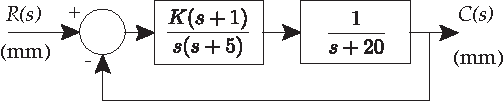
\includegraphics[width=2.75in]{ControlLoop2.pdf}
\caption{Control loop diagram}
\label{ControlLoop}
\end{center}
\end{figure}

Later on in the text: \dots We cite Figure \ref{ControlLoop} above.  Note the use of the \verb|\label{}| and \verb|\ref{}|.

Here are some numbered equations, with a reference.
\begin{equation}
T(s)=\frac{C(s)}{R(s)}=\frac{G(s)}{1+G(s)H(s)}
\label{eTF}
\end{equation}
\begin{equation}
\ket{f(x)} = \frac{1}{\sqrt{r}}\sum_{\ell=0}^{r-1}e^{2\pi i \ell/r}\ket{\hat{f}(\ell)}
\label{eFT}
\end{equation}

Elsewhere in  the text the equations \ref{eTF} and \ref{eFT} are cited. Note the use of the \verb|\label{}| and \verb|\ref{}|.

\vspace{.167in}
Here is an inline equation $f(t)=m\dot{v}(t)$. 
 
\vspace{.167in}
Some citations \cite{Bendat1971}, \cite{PhysRev.104.563}, \cite{Oppenheim1975}, and \cite{Papoulis1965}. 
 
\vspace{.167in}
A good \LaTeX\ reference is \cite{Lamport1994}.  See References.

\vspace{.167in}
The \verb|tabular| environment is tricky. 

But, it produces nice tables!

\vspace{.167in}
\begin{tabular}{|r||r@{--}l|p{1.25in}|}
\hline
\multicolumn{4}{|c|}{GG\&A Hoofed Stock}  \\  \hline  \hline
&\multicolumn{2}{c|}{Price}& \\ \cline{2-3}
\multicolumn{1}{|c||}{Year}
& \multicolumn{1}{r@{\,\vline\,}}{low}
& high & \multicolumn{1}{c|}{Comments} \\ \hline
1971 & 97 & 245 & Bad year. \\ \hline
72 & 245 &  245 & Light trading due to a heavy winter.  \\ \hline
73 & 245 & 2001 & No news was very good news this year. \\ \hline
\end{tabular}

\vspace{.5in}


\end{document}	%  <--- Here is where the document ends
